\documentclass[10pt,twocolumn,letterpaper]{article}

\usepackage[review]{cvpr}
\usepackage{times}
\usepackage{graphicx}
\usepackage{amsmath}
\usepackage{amssymb}
\usepackage{booktabs}
\usepackage{multirow}
\usepackage{algorithm}
\usepackage{algorithmic}
\usepackage{enumitem}
\usepackage{placeins}
\usepackage[pagebackref,breaklinks,colorlinks]{hyperref}

\setlist[itemize]{leftmargin=1.2em,itemsep=1pt,topsep=2pt,parsep=0pt}
\setlist[enumerate]{leftmargin=1.3em,itemsep=1pt,topsep=2pt,parsep=0pt}
\setlength{\textfloatsep}{7pt plus 1.5pt minus 1.5pt}
\setlength{\floatsep}{5pt plus 1.5pt minus 1.5pt}
\setlength{\dbltextfloatsep}{7pt plus 1.5pt minus 1.5pt}
\setlength{\dblfloatsep}{5pt plus 1.5pt minus 1.5pt}
\setlength{\abovecaptionskip}{3.5pt plus 1pt minus 1pt}
\setlength{\belowcaptionskip}{0pt}

\hypersetup{
  pdfkeywords={Vision-Language Models, Model Routing, Contextual Bandits, Multimodal Reasoning, Test-Time Compute Scaling, Efficient Inference}
}

\def\paperID{****}
\def\confName{CVPR}
\def\confYear{2027}

\title{CascadeRoute-VL: Taming the Reasoning Tax in Vision-Language Models via Online Contextual Bandit Routing}

\author{
Anonymous CVPR 2027 Submission \\
Paper ID: \paperID
}

\begin{document}

\maketitle

\begin{abstract}
Deploying Vision-Language Models (VLMs) at scale faces a critical accuracy-efficiency trade-off: compact models are fast but struggle on complex multi-step reasoning, whereas defaulting to massive frontier architectures or heavy test-time reasoning strategies incurs a Reasoning Tax---inflating token expenditure and latency while degrading performance on perception-dominant queries due to linguistic hallucination drift. Analyzing 30,540 multimodal queries across 14 diverse benchmarks and 17 contemporary VLMs (spanning 1B to 78B parameters and proprietary models), we observe a +17.24\% accuracy gap between the strongest static 72B frontier model (78.21\%) and an oracle selector (95.45\%), with compact ($\le 8\text{B}$) models accurately resolving 68.5\% of the queries on which the 72B model fails. To exploit this complementarity online without brittle offline retraining, we introduce \textbf{CascadeRoute-VL}, a contextual bandit routing framework that dynamically selects cost-efficient VLM configurations conditioned on joint visual, linguistic, and perceptual complexity cues (including luminance entropy, spatial edge density, and aspect ratio). CascadeRoute-VL employs Disjoint LinUCB with $O(d^2)$ Sherman-Morrison recursive updates, augmented with an offline \textbf{Warm-Start} initialization protocol to mitigate cold-start exploration penalties, \textbf{Budget-Aware Exploration Annealing} ($\alpha_t = \alpha_0 b_t$) with sublinear $\tilde{O}(d\sqrt{T})$ regret and asymptotic budget-feasibility guarantees, and a \textbf{Confidence-Guided Escalation Gate} to safeguard perception-critical predictions. Evaluations across large-scale multimodal benchmarks, distribution-shift stress tests (natural and STEM scenes to charts and dense OCR), and counterfactual Inverse Propensity Scoring (IPS/SNIPS) demonstrate that static offline supervised routers suffer severe out-of-distribution degradation without recovery, whereas CascadeRoute-VL continuously adapts online to achieve strong accuracy-efficiency trade-offs while substantially reducing token consumption and inference latency relative to monolithic frontier deployment.
\end{abstract}

% ============================================================================
\section{Introduction}
\label{sec:intro}
% ============================================================================

Deploying Vision-Language Models (VLMs) in production requires navigating a highly non-uniform cost-accuracy landscape across heterogeneous visual domains~\citep{huang2025vlrouterbench,bai2025qwen25vl,chen2024expanding}. Defaulting every incoming query to monolithic frontier models (such as 72B--78B open-weights checkpoints or proprietary APIs) or test-time reasoning architectures exacerbates compute expenditure while paradoxically harming fidelity on perception-heavy queries. Across 30,540 real queries from VL-RouterBench~\citep{huang2025vlrouterbench} spanning 14 benchmarks and 17 VLMs, \textbf{Qwen2.5-VL-72B} attains 78.21\% overall accuracy and fails on 6,655 queries. Crucially, a hindsight oracle over the 17-VLM pool reaches 95.45\% accuracy (\textbf{+17.24\% gap}), and compact models ($\le 8\text{B}$ parameters) successfully rescue \textbf{4,557 of those 6,655 failures (68.5\%)}.

\begin{figure*}[t]
\centering
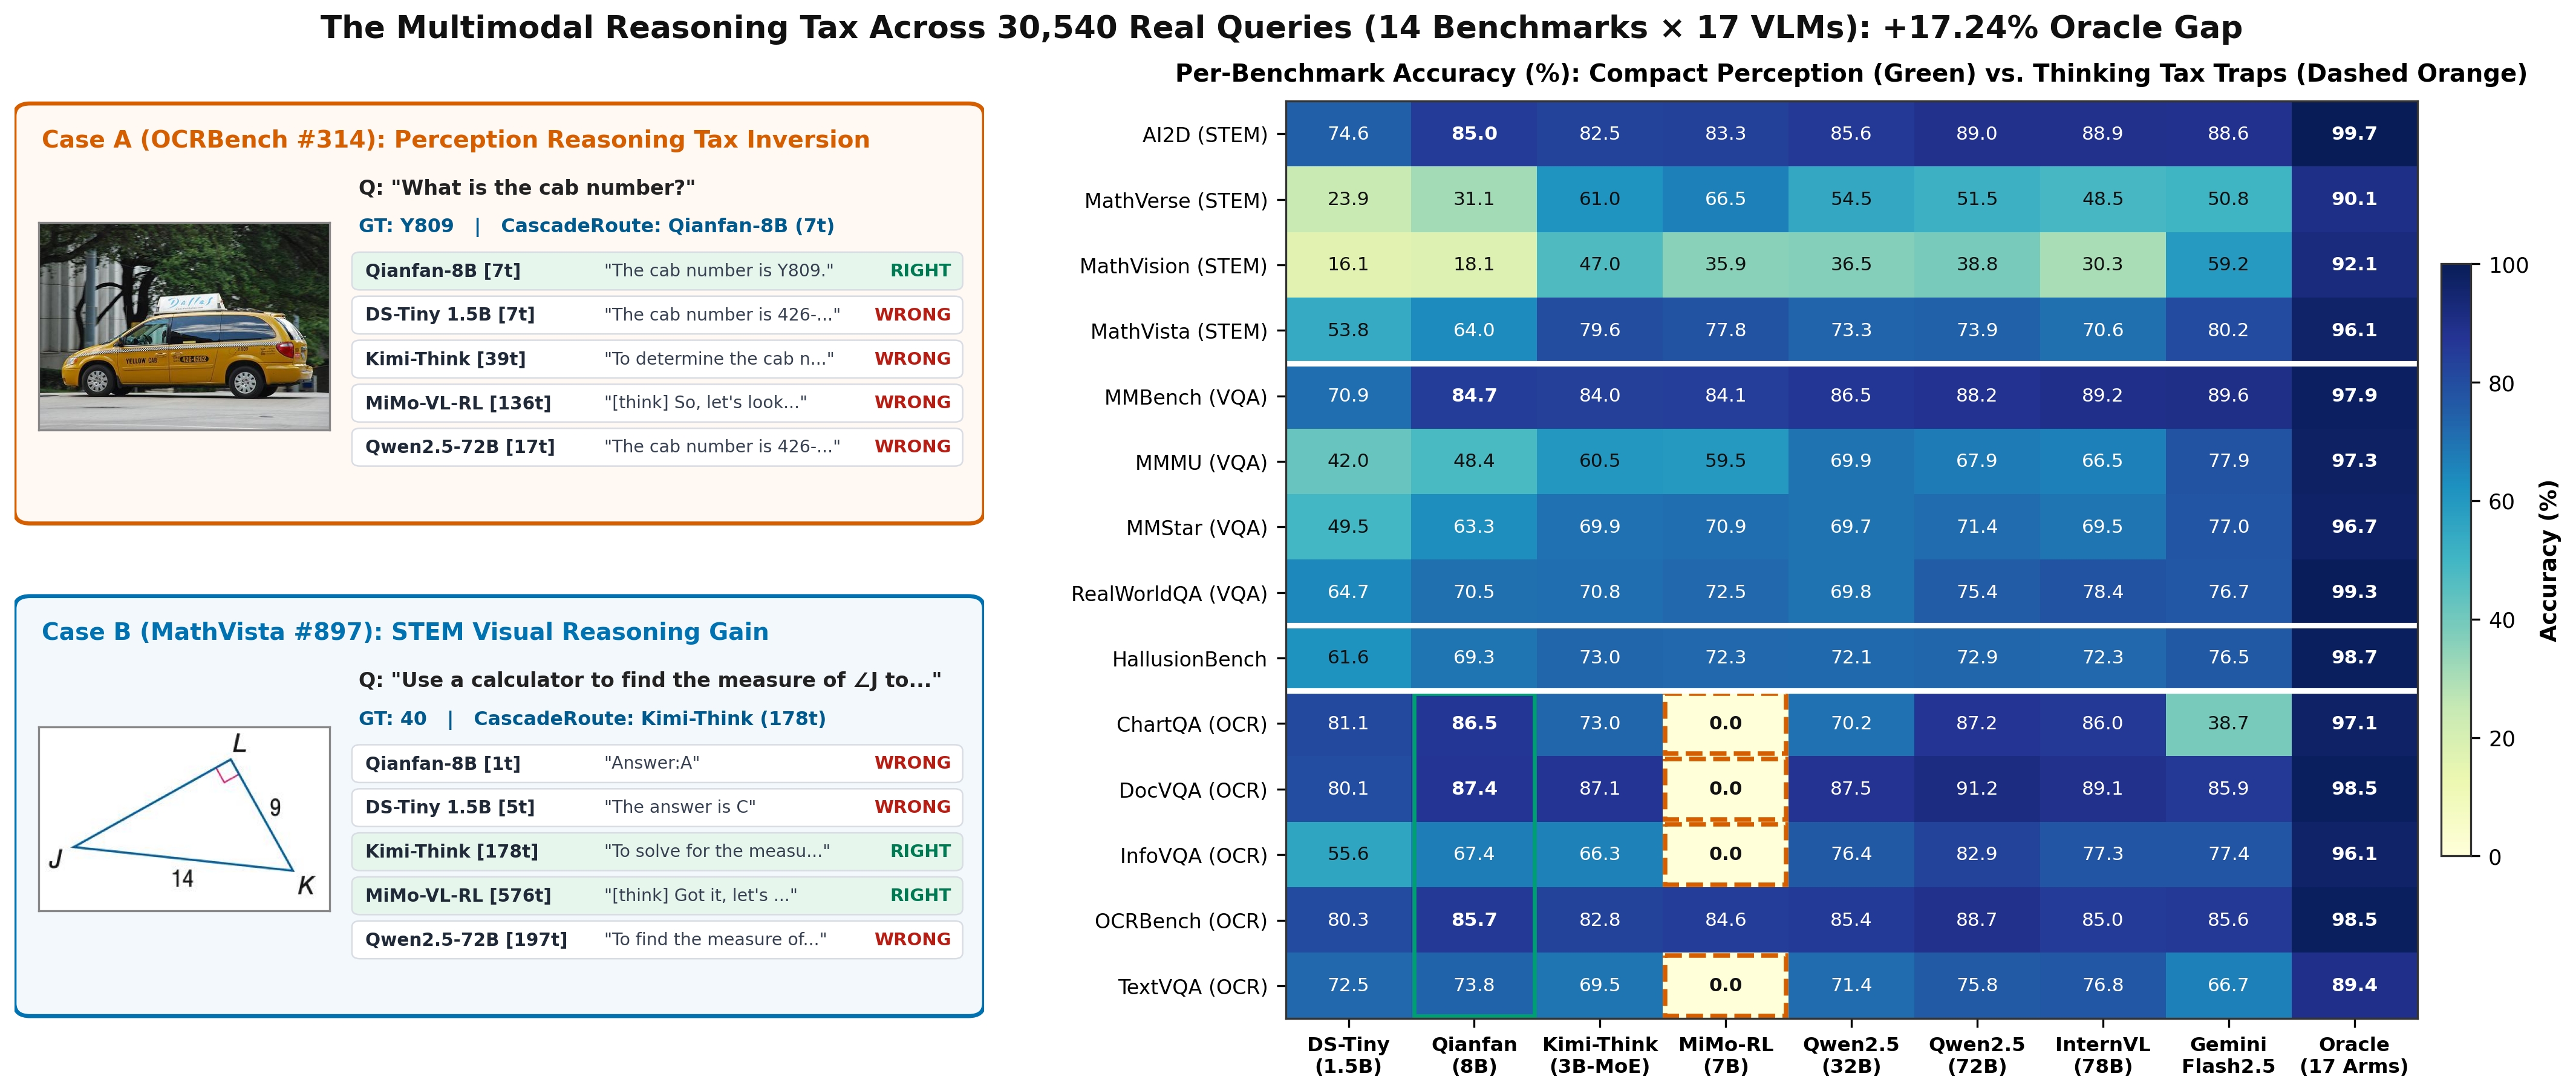
\includegraphics[width=0.93\textwidth]{../reports/figures/fig1_reasoning_tax_teaser.png}
\caption{\textbf{The Multimodal Reasoning Tax and Cross-Model Complementarity Across 30,540 Real Queries (14 Benchmarks $\times$ 17 VLMs).} \emph{Left (Top):} On OCRBench~\#314, compact \texttt{Qianfan-VL-8B} correctly reads cab number ``Y809'' in 7 tokens while \texttt{Qwen2.5-72B} (17 tok), \texttt{Kimi-Think} (39 tok), and \texttt{MiMo-VL-RL} (136 tok) over-rationalize and misread the fleet phone number or hallucinate. \emph{Left (Bottom):} On MathVista~\#897, compact models guess incorrectly in 1--5 tokens and \texttt{Qwen2.5-72B} confuses $\cos J$ with $\sin J$, whereas reasoning specialist \texttt{Kimi-VL-A3B-Thinking} solves the trigonometry exactly in 178 tokens. \emph{Right:} Across all 14 benchmarks, compact perception models excel on Charts/OCR (green box) while explicit \texttt{<think>} loops suffer severe extraction failures (dashed orange boxes on \texttt{MiMo-VL-7B-RL}).}
\label{fig:teaser}
\end{figure*}

Figure~\ref{fig:teaser} exposes the two opposing facets of this \textbf{Multimodal Reasoning Tax}. On STEM geometry and algorithmic counting problems (\eg, \texttt{MathVerse}, \texttt{MathVision}, \texttt{MathVista}~\citep{lu2024mathvista,zhang2024mathverse}), explicit reasoning yields decisive accuracy gains: 3B-active \texttt{Kimi-VL-A3B-Thinking}~\citep{kimi2025kimivl} reaches 79.6\% on \texttt{MathVista} and 47.0\% on \texttt{MathVision}, beating 72B \texttt{Qwen2.5-VL} (73.9\% and 38.8\%). Conversely, on fine-grained optical character recognition and visual grounding (\eg, \texttt{OCRBench}, \texttt{ChartQA}, \texttt{DocVQA}, \texttt{HallusionBench}~\citep{liu2024ocrbench,masry2022chartqa,mathew2021docvqa,guan2024hallusionbench}), unconstrained chain-of-thought reasoning frequently amplifies linguistic hallucination drift~\citep{shoby2026overthinking}: compact \texttt{Qianfan-VL-8B}~\citep{dong2025qianfanvl} delivers 86.5\% on \texttt{ChartQA} and 87.4\% on \texttt{DocVQA} using just 1.2--2.7 output tokens, while unconstrained \texttt{<think>} models burn dozens to hundreds of tokens and can even exhaust downstream answer extraction.

Existing routing solutions struggle to harness this complementarity safely under real deployment dynamics:
\begin{enumerate}
    \item \textbf{Static Offline Fragility:} Multi-label supervised routers in VL-RouterBench~\citep{huang2025vlrouterbench} and capability-profile classifiers such as ARMS~\citep{wang2026arms} assume stationary query distributions. In our strict cross-domain stress test (\texttt{General\_VQA + STEM} $\to$ unseen \texttt{Charts\_OCR + Hallucination}), a strong neural \texttt{MLP-Router} collapses from 72.77\% to \textbf{56.97\%} (\textbf{-15.80\%}) and never recovers.
    \item \textbf{Cold-Start Penalty \& Blindness to Perceptual Difficulty:} Naive online bandits suffer severe initial exploration regret (\eg, Cold LinUCB loses 5.91\% accuracy and costs +101\% more USD than our hybrid design), while text-only routers~\citep{ong2025routellm,chen2023frugalgpt} ignore visual complexity.
    \item \textbf{Benchmark Label Leakage:} Conditioning router features on oracle task/domain tags leaks benchmark identity during evaluation, masking failure modes when mixed real-world traffic arrives unlabelled.
\end{enumerate}

We resolve these limitations with \textbf{CascadeRoute-VL}, an online, zero-label contextual bandit router uniting four synergistic mechanisms:
\begin{itemize}
    \item \textbf{Zero-Leakage 904-d Multimodal Context State:} Fuses MiniLM-L6 text embeddings~\citep{wang2020minilm}, dual-scale DINOv2-ViT-S/14~\citep{oquab2024dinov2} + orthogonally projected ResNet-50~\citep{he2016deep} visual representations, and 8 unsupervised perceptual/linguistic complexity cues (entropy, Sobel edge density, aspect ratio, bright background ratio, symbolic cues) with provably bounded norm ($\|s_t\|_2 \le 0.9972$, max $0.8943 < 1$ empirically).
    \item \textbf{Warm-Started Disjoint LinUCB with Budget Annealing:} Combines $O(d^2)$ Sherman-Morrison recursive updates initialized via an offline ridge prior with dynamic budget-annealed exploration ($\alpha_t = \alpha_0 b_t$), attaining sublinear $\tilde{\mathcal{O}}(d\sqrt{KT})$ regret and asymptotic budget feasibility while adapting rapidly to distribution shifts.
    \item \textbf{Confidence-Guided Escalation Gate:} Evaluates compact primary selections using epistemic uncertainty $\sigma_a(s_t)$, cost-adjusted utility margins, unsupervised edge/math cues, and compact response-length bloat checks without peeking at ground-truth labels.
    \item \textbf{Large-Scale Rigor on 30,540 Real Queries:} Across 17 contemporary VLMs and 14 benchmarks, CascadeRoute-VL outperforms \texttt{Qwen2.5-VL-72B} by \textbf{+1.30\%} accuracy while cutting USD cost by \textbf{38.7\%} (up to \textbf{66.4\%} USD savings and \textbf{2.38$\times$} latency speedup in frugal mode), surpasses OOD \texttt{MLP-Router} within \textbf{$\sim$51} unseen queries (ending \textbf{+23.71\%} higher at 80.68\%), and passes unbiased IPS/SNIPS/DR counterfactual evaluation with 95\% bootstrap confidence intervals.
\end{itemize}

% ============================================================================
\section{Related Work}
\label{sec:related}
% ============================================================================

\textbf{LLM and VLM Routing.} Early routing work for language models demonstrated substantial inference savings through cascading (FrugalGPT~\citep{chen2023frugalgpt}), calibrated binary preference routing (RouteLLM~\citep{ong2025routellm}), dual-contrastive selection (RouterDC~\citep{chen2024routerdc}), and reward-guided ranking (Zooter~\citep{lu2024zooter}). Extending routing to multimodal models, VL-RouterBench~\citep{huang2025vlrouterbench} standardized evaluation over 14 vision-language benchmarks and benchmarked static supervised KNN, linear, and MLP routers. Subsequent methods incorporate static model capability profiles (ARMS~\citep{wang2026arms}) or episodic kNN retrieval memory (MHR-Router~\citep{zhu2026mhr}). Unlike static supervised routers that silently fail under domain shift, or heuristic retrieval stores lacking regret guarantees, CascadeRoute-VL pairs offline warm-start priors with theoretically grounded online contextual bandit adaptation and confidence-gated escalation.

\textbf{Multimodal Overthinking and Perceptual Grounding.} Recent analyses show that excessive test-time reasoning in VLMs can degrade accuracy by amplifying linguistic priors over grounded visual evidence~\citep{shoby2026overthinking}. Our large-scale matrix study across 17 VLMs—including explicit thinking architectures (\texttt{Kimi-VL-A3B-Thinking}~\citep{kimi2025kimivl}, \texttt{MiMo-VL-7B-RL}~\citep{xiaomi2025mimovl}) and perception-specialized compact models (\texttt{Qianfan-VL-8B}~\citep{dong2025qianfanvl}, \texttt{DeepSeek-VL2-Tiny}~\citep{wu2024deepseekvl2})—quantifies this dichotomy across reasoning-intensive STEM~\citep{lu2024mathvista,zhang2024mathverse,kembhavi2016ai2d} and OCR/hallucination~\citep{liu2024ocrbench,singh2019textvqa,guan2024hallusionbench} benchmarks. Rather than modifying VLM weights, CascadeRoute-VL mitigates the Reasoning Tax upfront at routing time.

\textbf{Contextual Bandits and Counterfactual Evaluation.} Disjoint LinUCB~\citep{li2010contextual} and confidence-ellipsoid linear bandits~\citep{abbasi2011improved} provide sharp sublinear regret bounds compared to classic non-contextual bandits~\citep{auer2002ucb} and deep heuristic policies~\citep{mnih2015dqn,agrawal2013thompson}. To validate routed policies cleanly from logged feedback without selection bias, Inverse Propensity Scoring (IPS), Self-Normalized IPS (SNIPS)~\citep{swaminathan2015self}, and Doubly Robust (DR) estimators~\citep{dudik2011doubly} provide finite-sample counterfactual confidence intervals, which we report alongside live online evaluations.

% ============================================================================
\section{Quantifying the Multimodal Reasoning Tax}
\label{sec:tax}
% ============================================================================

We analyze the complete outcome tensor $Y \in \{0,1\}^{N \times K}$ over $N = 30{,}540$ standardized queries across 14 benchmarks spanning four domains---\texttt{STEM} (\texttt{AI2D}, \texttt{MathVista}, \texttt{MathVerse}, \texttt{MathVision}; $N{=}8{,}332$), \texttt{General\_VQA} (\texttt{MMBench}, \texttt{MMMU}, \texttt{MMStar}, \texttt{RealWorldQA}; $N{=}4{,}607$~\citep{liu2024mmbench,yue2024mmmu,chen2024mmstar}), \texttt{Hallucination} (\texttt{HallusionBench}; $N{=}951$), and \texttt{Charts\_OCR} (\texttt{ChartQA}, \texttt{DocVQA}, \texttt{InfoVQA}, \texttt{OCRBench}, \texttt{TextVQA}; $N{=}16{,}650$~\citep{mathew2022infographicvqa,singh2019textvqa})---paired with $K=17$ VLMs from 1B to 78B parameters and proprietary APIs (\texttt{GPT-4o}, \texttt{GeminiFlash2.5}). Per-query costs and latencies are reconstructed directly from the $238$ raw inference transcripts using \texttt{cl100k\_base} tokenization ($+256$ visual tokens per image) and benchmark pricing (profiles in Supplementary Sec.~S2).

\begin{figure*}[t]
\centering
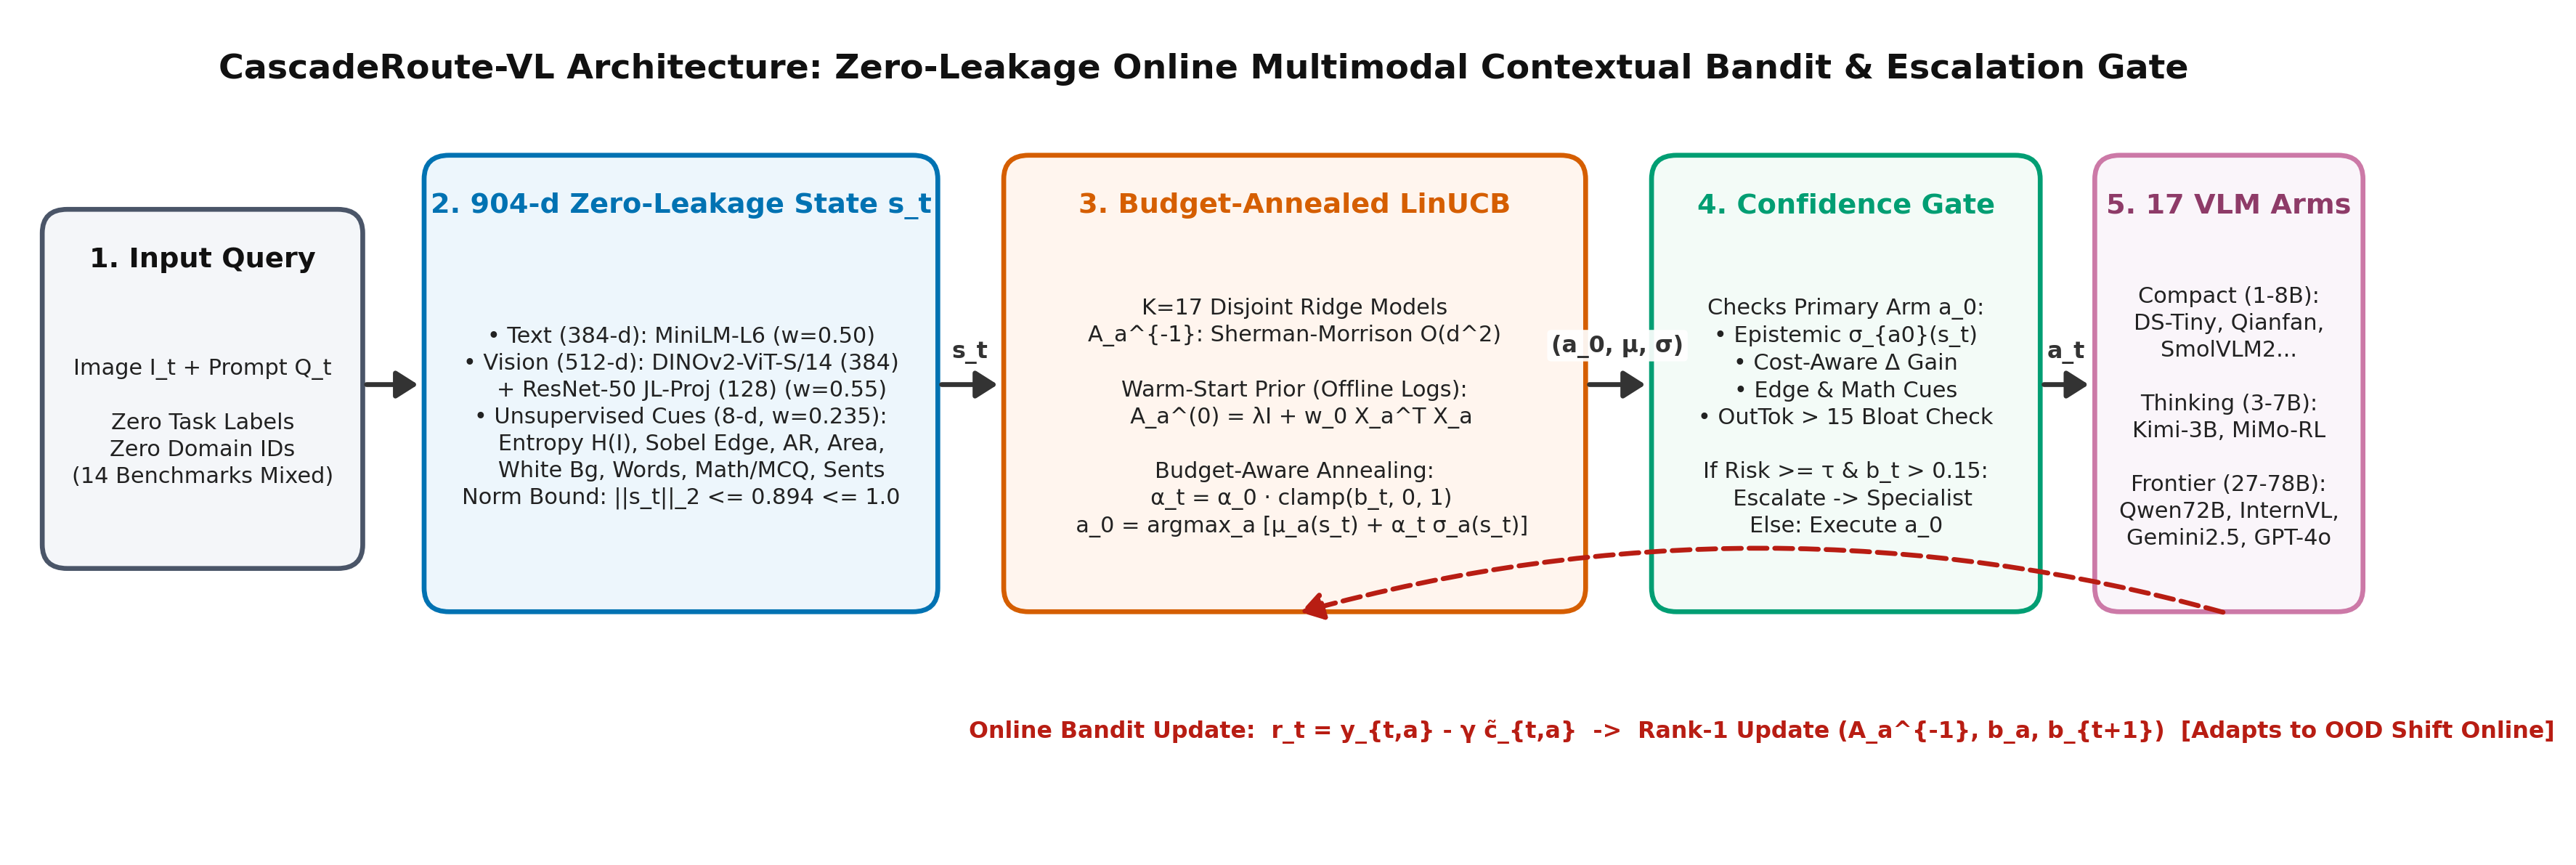
\includegraphics[width=0.88\textwidth]{../reports/figures/fig2_architecture.png}
\caption{\textbf{CascadeRoute-VL Architecture.} Input image-question pairs are encoded into a strictly zero-leakage 904-d context vector $s_t$ ($\|s_t\|_2 \le 0.9972$ analytically, max $0.8943 < 1$ empirically) fusing MiniLM-L6 text semantics, dual-scale DINOv2+ResNet-50 vision embeddings, and 8 unsupervised perceptual/linguistic cues. Budget-annealed Disjoint LinUCB initialized from an offline warm-start prior scores all 17 VLM arms, while the Confidence Gate safeguards uncertain compact predictions before real-time Sherman-Morrison $O(d^2)$ online updates refine policy weights under distribution shift.}
\label{fig:architecture}
\end{figure*}

Three structural properties motivate online multimodal routing:
\begin{enumerate}
    \item \textbf{Massive Untapped Complementarity (+17.24\% Gap):} While \texttt{Qwen2.5-VL-72B} leads all individual models at 78.21\% overall accuracy (\$0.2626/1k queries), an oracle arm selector reaches \textbf{95.45\%}, rescuing 5,266 of the 6,655 frontier failures (79.1\%). Crucially, compact models ($\le 8\text{B}$) solve \textbf{68.5\%} (4,557/6,655) of 72B failures---led by \texttt{Kimi-VL-A3B-Thinking} (2,324 rescues), \texttt{Qianfan-VL-8B} (1,789), and \texttt{DeepSeek-VL2-Tiny} (1,689).
    \item \textbf{Reasoning Inversion Under Perception Load:} On \texttt{Charts\_OCR}, concise perception specialists dominate: \texttt{Qianfan-VL-8B} achieves 86.48\% on \texttt{ChartQA} (1.2 avg output tokens), 87.42\% on \texttt{DocVQA} (2.7 tok), and 85.70\% on \texttt{OCRBench} (4.6 tok), closely rivaling 72B at $\sim 5\times$ lower cost and $\sim 8.8\times$ lower latency. Conversely, verbose reasoning degrades perceptual precision (Fig.~\ref{fig:teaser}a) or causes complete downstream format/length breakdown: \texttt{MiMo-VL-7B-RL} generates \texttt{<think>} chains on 100\% of queries (mean 237.4 output tokens) and scores \textbf{0.0\%} extracted accuracy across four OCR benchmarks (\texttt{ChartQA}, \texttt{DocVQA}, \texttt{InfoVQA}, \texttt{TextVQA}).
    \item \textbf{Visual/Text Complexity Signals Enable Zero-Label Routing:} Unsupervised cues cleanly separate regimes without ground-truth domain tags: math benchmarks exhibit low luminance entropy (2.00--3.72 bits), high white-background ratios (0.60--0.89), and elevated symbolic density (0.27--0.36), whereas natural scene OCR (\texttt{TextVQA}) shows high entropy (7.10 bits) and dense edge structure.
\end{enumerate}

% ============================================================================
\section{CascadeRoute-VL Framework}
\label{sec:method}
% ============================================================================

Figure~\ref{fig:architecture} illustrates the complete routing loop. At discrete step $t \in \{1,\dots,T\}$, an unlabelled multimodal query $(I_t, Q_t)$ arrives without task or dataset identifiers. The router chooses an arm $a_t \in \mathcal{A} = \{1,\dots,K\}$ ($K{=}17$), executes inference to observe correctness $y_{t,a_t} \in \{0,1\}$, USD cost $c_{t,a_t} \ge 0$, and output length $o_{t,a_t}$, and updates its contextual posterior online.

\subsection{Zero-Leakage Multimodal Context State}
\label{sec:state}

To satisfy norm boundedness required for linear bandit concentration guarantees while preventing benchmark leakage, we construct $s_t \in \mathbb{R}^{d}$ ($d{=}904$) purely from the raw input pair $(I_t, Q_t)$:
\begin{equation}
s_t = \left[\, w_q \hat{q}_t \;\|\; w_v \hat{v}_t \;\|\; w_p p_t \,\right] \in \mathbb{R}^{904},
\end{equation}
where weights $(w_q, w_v, w_p) = (0.50, 0.55, 0.235)$ combine:
\begin{itemize}
    \item \textbf{Linguistic Semantics ($\hat{q}_t \in \mathbb{R}^{384}$):} $L_2$-normalized \texttt{all-MiniLM-L6-v2} embedding capturing reasoning intent~\citep{wang2020minilm}.
    \item \textbf{Dual-Scale Vision ($\hat{v}_t \in \mathbb{R}^{512}$):} $L_2$-normalized concatenation of global structural semantics from frozen \texttt{DINOv2-ViT-S/14} \texttt{[CLS]} (384-d)~\citep{oquab2024dinov2} and texture/layout detail from a fixed deterministic Johnson-Lindenstrauss orthonormal projection ($2048 \to 128$) of \texttt{ResNet-50} GAP~\citep{he2016deep}.
    \item \textbf{Unsupervised Perceptual \& Syntactic Cues ($p_t \in [0,1]^8$):} Normalized image luminance Shannon entropy $H(I_t)/8$, Sobel edge gradient density $\nabla(I_t)$, logarithmic aspect ratio encoding $\frac{1}{\pi}\arctan(\ln(W/H)) + 0.5$, normalized log area $\text{clip}(\log_{10}(WH)/7, 0, 1)$, flat white background pixel fraction ($L > 235/255$), clipped prompt word count, symbolic/digit/MCQ density, and sentence count.
\end{itemize}
Unlike static routers relying on domain one-hot vectors, every coordinate of $p_t$ lies strictly in $[0,1]$, ensuring an explicit Euclidean bound across all inputs without dataset metadata:
\begin{equation}
\|s_t\|_2 \le \sqrt{w_q^2 + w_v^2 + 8 w_p^2} = \sqrt{0.9943} < 1.0.
\end{equation}

\subsection{Warm-Started Disjoint LinUCB \& Cost Reward}
\label{sec:linucb}

We define the cost-adjusted scalar reward for selecting arm $a$ on query $t$ with cost sensitivity parameter $\gamma \ge 0$ as:
\begin{equation}
r_{t,a} = y_{t,a} - \gamma \tilde{c}_{t,a}, \qquad \tilde{c}_{t,a} = \text{clip}\!\left(\frac{c_{t,a}}{c_{90}}, 0, 2.5\right),
\end{equation}
where $c_{90} = \$0.000329$ is the 90th percentile training-arm mean cost, keeping normalized costs invariant across heterogeneous currency scales. Modeling $\mathbb{E}[r_{t,a} \mid s_t] = \theta_a^\top s_t$, we maintain per-arm inverse regularized design matrices $A_a^{-1} \in \mathbb{R}^{d \times d}$ and response vectors $b_a \in \mathbb{R}^d$, yielding ridge parameters $\hat{\theta}_a = A_a^{-1} b_a$ and epistemic uncertainty $\sigma_a(s_t) = \sqrt{s_t^\top A_a^{-1} s_t}$.

\textbf{Offline Warm-Start Prior.} Initializing $A_a = \lambda I_d$ online incurs heavy early exploration regret over $K{=}17$ VLMs. Given offline training interactions $\mathcal{D}_{\text{off}} = \{(s_i, a_i, r_i)\}_{i=1}^{N_{\text{off}}}$ scaled by prior weight $w_0 \in (0, 1]$ to preserve plasticity under non-stationarity, we initialize:
\begin{equation}
A_a^{(0)} = \lambda I_d + w_0 \!\!\sum_{i:\, a_i = a} s_i s_i^\top, \qquad b_a^{(0)} = w_0 \!\!\sum_{i:\, a_i = a} r_i s_i.
\label{eq:warmstart}
\end{equation}

\textbf{Online Sherman-Morrison Updates.} Upon observing live feedback $r_t$ for executed arm $a$, $A_a^{-1}$ is updated in exact $O(d^2)$ time without $O(d^3)$ matrix inversion:
\begin{equation}
A_a^{-1} \leftarrow A_a^{-1} - \frac{(A_a^{-1} s_t)(A_a^{-1} s_t)^\top}{1 + s_t^\top A_a^{-1} s_t}, \qquad b_a \leftarrow b_a + r_t s_t.
\label{eq:sherman}
\end{equation}

\subsection{Budget Annealing and Confidence Escalation Gate}
\label{sec:gate}

Given total session USD budget $B_{\max}$ and cumulative expenditure $C_{t-1} = \sum_{j=1}^{t-1} c_{j}$, the normalized remaining budget fraction is $b_t = \max(0, \min(1, (B_{\max} - C_{t-1}) / B_{\max}))$. We modulate exploration via \textbf{Budget-Aware Exploration Annealing}:
\begin{equation}
\alpha_t = \alpha_0 \cdot b_t, \qquad a_0 = \arg\max_{a \in \mathcal{A}} \left( \hat{\theta}_a^\top s_t + \alpha_t \sigma_a(s_t) \right).
\label{eq:anneal}
\end{equation}
When budget is plentiful ($b_t \approx 1$), CascadeRoute-VL actively explores specialist VLMs; as budget tightens ($b_t \to 0$), $\alpha_t \to 0$ collapses exploration bonuses onto high-utility compact models.

\textbf{Confidence-Guided Escalation Gate.} When primary choice $a_0$ belongs to the compact tier ($\le 8\text{B}$ direct models) and remaining budget satisfies $b_t > b_{\min}$ ($b_{\min}{=}0.15$), we run $a_0$ and inspect post-call output token count $o_{t,a_0}$ alongside zero-oracle bandit signals (never accessing ground-truth labels). First, recovering cost-adjusted quality estimates $\hat{\mu}_a = \hat{\theta}_a^\top s_t + \gamma \bar{c}_a$, the gate identifies the utility-optimal specialist/frontier fallback $a^* \in \mathcal{F}$ (\texttt{Kimi-3B-Think}, \texttt{Qwen2.5-72B}, \texttt{InternVL2.5-78B}, \texttt{GeminiFlash2.5}) maximizing $\hat{\mu}_a - \kappa \gamma \bar{c}_a$ ($\kappa{=}0.22$). With effective gain $\Delta_{\text{eff}} = (\hat{\mu}_{a^*} - \hat{\mu}_{a_0}) - \kappa \gamma \max(0, \bar{c}_{a^*} - \bar{c}_{a_0})$, the gate computes risk score:
\begin{equation}
\begin{aligned}
\rho_t = \Delta_{\text{eff}} &+ 0.25\,\sigma_{a_0}(s_t) + 0.06\,\nabla(I_t) \\
&+ 0.06\,\psi_{\text{math}}(Q_t) + 0.05\,\mathbb{I}[o_{t,a_0} > 15],
\end{aligned}
\end{equation}
escalating to $a^*$ whenever $\hat{\mu}_{a_0} < p_{\text{cap}}$ ($0.78$), $\Delta_{\text{eff}} \ge \tau_m$ ($0.025$), and $\rho_t \ge \tau_u$ ($0.12$). All cascade tokens, latencies, and rewards are truthfully billed to both arms before executing Eq.~\eqref{eq:sherman}. \emph{(Live serving backbones can additionally evaluate visual perturbation stability $S_{\text{OT}} = 1 - \text{Jaccard}(A_1, A_2)$ directly~\citep{shoby2026overthinking}.)} Algorithm~\ref{alg:cascaderoute} summarizes the complete procedure.

\begin{algorithm}[t]
\caption{CascadeRoute-VL Online Inference \& Update}
\label{alg:cascaderoute}
\begin{algorithmic}[1]
\REQUIRE Arms $\mathcal{A}$ ($|\mathcal{A}|=K$), prior $(\mathcal{D}_{\text{off}}, w_0, \lambda)$, $\alpha_0$, $\gamma$, budget $B_{\max}$, fallback pool $\mathcal{F}$
\STATE Initialize $(A_a^{(0)})^{-1}, b_a^{(0)}, \hat{\theta}_a^{(0)}$ via Eq.~\eqref{eq:warmstart}; $C_0 \leftarrow 0$
\FOR{$t = 1, \dots, T$}
    \STATE Encode $s_t \in \mathbb{R}^{904}$ from $(I_t, Q_t)$ (zero task labels); set $b_t \leftarrow \text{clip}((B_{\max}-C_{t-1})/B_{\max}, 0, 1)$
    \STATE Compute $\alpha_t \leftarrow \alpha_0 b_t$, $\hat{\theta}_a^\top s_t$, $\sigma_a(s_t)$, and $a_0 \leftarrow \arg\max_a (\hat{\theta}_a^\top s_t + \alpha_t \sigma_a(s_t))$
    \STATE Query VLM $a_0$, observe outcome $y_{t,a_0}$, cost $c_{t,a_0}$, output length $o_{t,a_0}$
    \STATE Update $(A_{a_0}^{-1}, b_{a_0}, \hat{\theta}_{a_0})$ with $r_{t,a_0} = y_{t,a_0} - \gamma \tilde{c}_{t,a_0}$ via Eq.~\eqref{eq:sherman}
    \IF{$a_0 \in \mathcal{A}_{\text{compact}}$ \textbf{and} $b_t > 0.15$ \textbf{and} GateTriggers($\hat{\mu}, \sigma_{a_0}, p_t, o_{t,a_0}, \mathcal{F}$)}
        \STATE Escalate to $a^* \in \mathcal{F}$, observe $(y_{t,a^*}, c_{t,a^*})$, bill $C_t \leftarrow C_{t-1} + c_{t,a_0} + c_{t,a^*}$
        \STATE Update $(A_{a^*}^{-1}, b_{a^*}, \hat{\theta}_{a^*})$ with $r_{t,a^*}$ via Eq.~\eqref{eq:sherman}; output prediction of $a^*$
    \ELSE
        \STATE Bill $C_t \leftarrow C_{t-1} + c_{t,a_0}$; output prediction of $a_0$
    \ENDIF
\ENDFOR
\end{algorithmic}
\end{algorithm}

\subsection{Theoretical Guarantees}
\label{sec:theory}

Full proofs of all lemmas and theorems are provided in Supplementary Sec.~S1.

\textbf{Lemma 1 (Bounded Context Space).} \emph{Under $(w_q, w_v, w_p) = (0.50, 0.55, 0.235)$, all encoded queries satisfy $\|s_t\|_2 \le 0.9972 < 1$.}

\textbf{Lemma 2 (Sub-Gaussian Reward Noise).} \emph{With $y_{t,a} \in \{0,1\}$ and $\tilde{c}_{t,a} \in [0, 2.5]$, rewards satisfy $r_{t,a} \in [-2.5\gamma, 1]$, so reward noise $\eta_t = r_{t,a} - \mathbb{E}[r_{t,a} \mid s_t]$ is conditionally $\nu$-sub-Gaussian with $\nu = (1 + 2.5\gamma)/2$.}

\textbf{Theorem 1 (Disjoint Multimodal Regret Bound \& OOD Prior Decay).} \emph{Suppose $\|\theta_a\|_2 \le S$ for all $a \in \mathcal{A}$, and exploration scales satisfy $\alpha_0 \ge \nu \sqrt{d \ln((1 + T w_0^{-1}\lambda_{\max})/\delta)} + \sqrt{\lambda} S$. Applying Cauchy-Schwarz and the elliptical potential lemma across disjoint arm visit counts $\sum_{a=1}^K T_a = T$ (via $\sum_{a=1}^K \sqrt{T_a} \le \sqrt{K T}$), with probability at least $1-\delta$, cumulative pseudo-regret satisfies:}
\begin{equation}
R_T \le 2\alpha_0 \sqrt{2 d K T \ln\!\left(1 + \frac{T}{d \lambda}\right)} + \mathcal{O}(K) = \tilde{\mathcal{O}}(d \sqrt{K T}).
\end{equation}
\emph{Moreover, under an out-of-distribution shift where static offline classifiers incur linear regret $\Omega(\Delta_{\text{shift}} T)$, the offline warm-start regularizer scaled by $w_0$ decays as $\mathcal{O}(w_0 \Delta_{\text{shift}} / n_{t,a})$ while online Sherman-Morrison observations drive cumulative OOD regret sublinearly.}

\textbf{Theorem 2 (Asymptotic Budget Feasibility).} \emph{For any positive budget $B_{\max}$, under annealed exploration $\alpha_t = \alpha_0 b_t$ and the confidence gate cutoff $b_t > 0.15$, as remaining reserves approach zero ($b_t \to 0^+$), exploration vanishes and decisions collapse to the cost-penalized ridge exploiter $\arg\max_a \hat{\theta}_a^\top s_t$ with escalation disabled, preventing runaway budget overruns.}

% ============================================================================
\section{Experimental Evaluation}
\label{sec:experiments}
% ============================================================================

\subsection{Setup, Baselines, and Protocol}
\label{sec:setup}

We use the exact official VL-RouterBench split across 30,540 queries: \texttt{Train} ($N{=}21{,}378$), \texttt{Dev} ($N{=}3{,}054$), and held-out \texttt{Test} ($N{=}6{,}108$). All hyperparameters for \textbf{CascadeRoute-VL} ($w_0{=}0.20, \lambda{=}4.0, \alpha_0{=}0.10$) are calibrated strictly on \texttt{Dev} with zero \texttt{Test} peeking, and online evaluations average across 5 random stream permutations (seeds 42--46).

We compare 20 baselines and variants: (1)~\textbf{Static VLMs} (\texttt{Qwen2.5-VL-72B}, \texttt{InternVL2.5-78B}, \texttt{Qwen2.5-VL-32B}, \texttt{Kimi-VL-A3B-Thinking}, \texttt{GeminiFlash2.5}, \texttt{Qianfan-VL-8B}, \texttt{DeepSeek-VL2-Tiny}); (2)~\textbf{Static Offline Routers} (\texttt{Offline-Linear}, \texttt{KNN-Router} $k{=}15$, \texttt{ARMS-Router}~\citep{wang2026arms}, GPU 3-layer \texttt{MLP-Router} with LayerNorm+SiLU+BCE); (3)~\textbf{Sequential Cascade} (4-tier \texttt{FrugalGPT-Cascade}~\citep{chen2023frugalgpt} at $\tau{=}0.72$); (4)~\textbf{Online \& Retrieval Bandits} (\texttt{Epsilon-Greedy}, \texttt{UCB1}~\citep{auer2002ucb}, \texttt{Thompson-Sampling}~\citep{agrawal2013thompson}, \texttt{DQN-Router}~\citep{mnih2015dqn}, \texttt{MHR-Router}~\citep{zhu2026mhr}, cold \texttt{LinUCB}); and (5)~\textbf{CascadeRoute-VL (Ours)} at $\gamma{=}0.08$ and $\gamma{=}0.30$.

\subsection{Main Held-Out Benchmark and Pareto Frontiers}
\label{sec:main_res}

\begin{table*}[t]
\centering
\scriptsize
\setlength{\tabcolsep}{3.6pt}
\renewcommand{\arraystretch}{0.94}
\caption{\textbf{Held-Out Test Benchmark Comparison ($N{=}6{,}108$, 17 VLMs, 5 Seeds for Stochastic Policies).} CascadeRoute-VL ($\gamma{=}0.08$) outperforms monolithic 72B by +1.30\% accuracy while cutting USD cost by 38.7\%; frugal mode ($\gamma{=}0.30$) cuts cost by 66.4\% with 2.38$\times$ latency speedup.}
\label{tab:main_benchmark}
\resizebox{\textwidth}{!}{%
\begin{tabular}{llccccccc}
\toprule
\textbf{Algorithm} & \textbf{Category} & \textbf{Acc (\%)} & \textbf{Avg Tok} & \textbf{Out Tok} & \textbf{Latency (s)} & \textbf{Cost / 1k (\$)} & \textbf{USD Saved} & \textbf{Cum. Regret} \\
\midrule
\texttt{Qwen2.5-VL-72B}~\citep{bai2025qwen25vl} & Static VLM & 77.29 & 309.8 & 31.7 & 1.959 & \$0.2605 & 0.0\% & 1092.0 \\
\texttt{InternVL2.5-78B}~\citep{chen2024expanding} & Static VLM & 76.20 & 293.5 & 15.4 & 1.328 & \$0.3012 & -15.6\% & 1159.0 \\
\texttt{Qwen2.5-VL-32B} & Static VLM & 74.28 & 379.0 & 100.8 & 3.306 & \$0.1718 & 34.1\% & 1276.0 \\
\texttt{Kimi-VL-3B-Think}~\citep{kimi2025kimivl} & Static VLM & 72.86 & 335.3 & 57.1 & 0.741 & \$0.0699 & 73.2\% & 1363.0 \\
\texttt{GeminiFlash2.5} & Static API & 72.33 & 393.0 & 114.8 & 1.364 & \$0.3590 & -37.8\% & 1395.0 \\
\texttt{Qianfan-VL-8B}~\citep{dong2025qianfanvl} & Static VLM & 69.88 & 282.2 & 4.1 & 0.228 & \$0.0511 & 80.4\% & 1545.0 \\
\texttt{DeepSeek-VL2-Tiny}~\citep{wu2024deepseekvl2} & Static VLM & 62.57 & 285.5 & 7.3 & \textbf{0.144} & \textbf{\$0.0143} & \textbf{94.5\%} & 1991.0 \\
\midrule
\texttt{Offline-Linear} & Offline Router & 78.21 & 384.3 & 106.2 & 1.721 & \$0.1777 & 31.8\% & 1036.0 \\
\texttt{KNN-Router} ($k{=}15$) & Offline Router & 78.31 & 361.8 & 83.7 & 1.444 & \$0.1306 & 49.9\% & 1030.0 \\
\texttt{ARMS-Router}~\citep{wang2026arms} & Offline Router & 78.80 & 369.0 & 90.8 & 1.306 & \$0.2190 & 16.0\% & 1000.0 \\
\texttt{MLP-Router}~\citep{huang2025vlrouterbench} & Offline Router & \textbf{79.85} & 400.4 & 122.2 & 1.844 & \$0.1854 & 28.8\% & \textbf{936.0} \\
\texttt{FrugalGPT-Cascade}~\citep{chen2023frugalgpt} & Seq. Cascade & 73.23 & 725.8 & 69.7 & 1.719 & \$0.1704 & 34.6\% & 1340.0 \\
\midrule
\texttt{Epsilon-Greedy} ($\epsilon{=}0.1$) & Online Bandit & 69.25 $\pm$ 3.74 & 364.2 & 86.0 & 1.445 & \$0.2803 & -7.6\% & 1583.2 \\
\texttt{UCB1}~\citep{auer2002ucb} & Online Bandit & 68.42 $\pm$ 0.75 & 321.6 & 43.4 & 1.271 & \$0.1622 & 37.7\% & 1634.0 \\
\texttt{Thompson Sampling}~\citep{agrawal2013thompson} & Online Bandit & 69.50 $\pm$ 0.86 & 340.3 & 62.2 & 1.396 & \$0.1595 & 38.8\% & 1568.0 \\
\texttt{DQN-Router}~\citep{mnih2015dqn} & Online Bandit & 72.96 $\pm$ 1.02 & 335.5 & 57.3 & 1.421 & \$0.1845 & 29.2\% & 1356.4 \\
\texttt{MHR-Router}~\citep{zhu2026mhr} & Retrieval Bandit & 71.48 $\pm$ 0.51 & 346.4 & 68.2 & 1.333 & \$0.1247 & 52.1\% & 1446.8 \\
\texttt{LinUCB (Cold Online)} & Online Bandit & 72.68 $\pm$ 1.71 & 363.0 & 84.9 & 1.535 & \$0.3220 & -23.6\% & 1373.8 \\
\midrule
\textbf{CascadeRoute-VL (Frugal $\gamma{=}0.30$)} & \textbf{Proposed} & 76.13 $\pm$ 0.21 & \textbf{360.5} & \textbf{51.1} & \textbf{0.824} & \textbf{\$0.0876} & \textbf{66.4\%} & 1162.8 \\
\textbf{CascadeRoute-VL (Full, $\gamma{=}0.08$)} & \textbf{Proposed} & \textbf{78.59 $\pm$ 0.12} & 370.8 & 91.9 & 1.550 & \$0.1598 & 38.7\% & \textbf{1013.0} \\
\midrule
\texttt{Oracle (Hindsight 17-Arm)} & Upper Bound & 95.17 & 296.5 & 18.3 & 0.339 & \$0.0348 & 86.6\% & 0.0 \\
\bottomrule
\end{tabular}%
}
\end{table*}

\begin{figure*}[t]
\centering
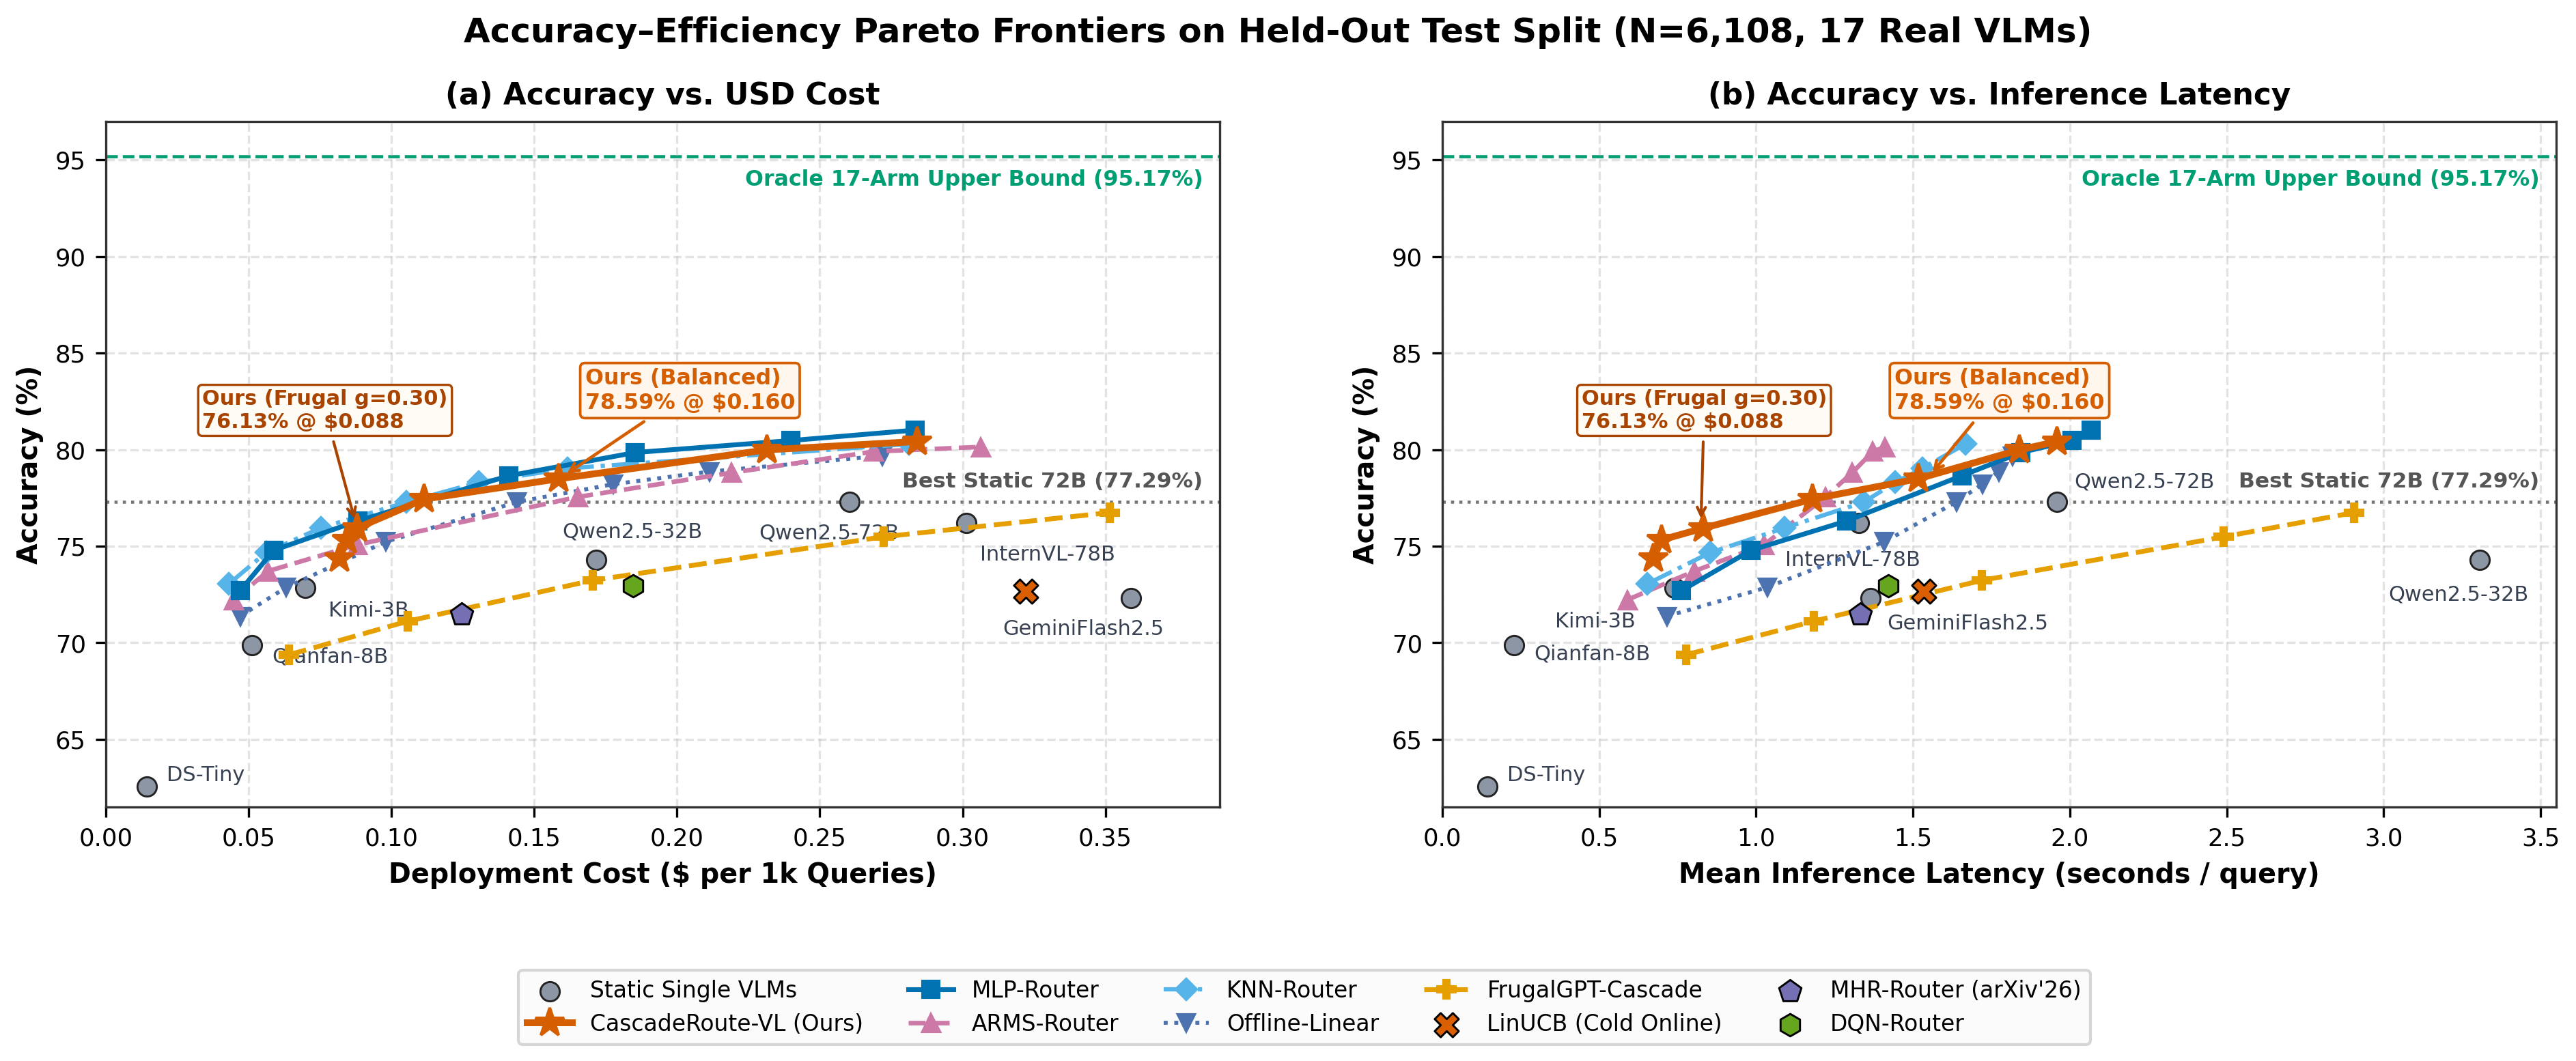
\includegraphics[width=0.89\textwidth]{../reports/figures/fig3_pareto_frontier.png}
\caption{\textbf{Accuracy vs.\ Cost and Inference Latency Pareto Frontiers on Held-Out Test ($N{=}6{,}108$).} Sweeping $\gamma \in [0, 0.9]$ shows CascadeRoute-VL spans a monotone frontier exceeding monolithic 72B while staying cheaper and faster than offline routers and \texttt{FrugalGPT}.}
\label{fig:pareto}
\end{figure*}

Table~\ref{tab:main_benchmark} and Figure~\ref{fig:pareto} summarize held-out test results across all 17 VLMs:
\begin{itemize}
    \item \textbf{Monolithic 72B \& Online Bandit Gains:} At balanced $\gamma{=}0.08$, \texttt{CascadeRoute-VL} achieves \textbf{78.59\% $\pm$ 0.12\%} at \$0.1598/1k queries---\textbf{+1.30\%} above \texttt{Qwen2.5-VL-72B} (77.29\%; paired $t$-test $p{=}0.015$ on seed~42) with \textbf{38.7\% USD saved} ($p{=}9.49\times 10^{-275}$) and $1.26\times$ speedup. It significantly beats \texttt{Cold LinUCB} (+5.91\%, Bonferroni $p{=}1.07\times 10^{-22}$), \texttt{MHR-Router} (+7.11\%, $p{=}5.17\times 10^{-32}$), \texttt{DQN} (+5.63\%), and \texttt{FrugalGPT} (+5.36\%, $p{=}3.34\times 10^{-25}$).
    \item \textbf{Frugal Mode ($\gamma{=}0.30$):} Achieves \textbf{76.13\% $\pm$ 0.21\%} at \textbf{\$0.0876/1k} and \textbf{0.824s}---\textbf{66.4\% USD savings} and \textbf{2.38$\times$ speedup} vs.\ 72B, outperforming \texttt{FrugalGPT} (73.23\%) at nearly half the cost and tokens (360.5 vs.\ 725.8).
    \item \textbf{Pareto Frontier vs.\ Offline Classifiers:} On i.i.d.\ splits, static \texttt{MLP-Router} hits 79.85\% at higher cost (\$0.1854/1k, $p{=}6.30\times 10^{-12}$) and latency (1.844s). Across $\gamma \in [0, 0.9]$, CascadeRoute-VL matches offline routers for $\gamma \le 0.15$ and beats \texttt{MLP-Router} by +1.67\% (74.36\% vs.\ 72.69\%) at $\gamma{=}0.90$, while preserving online adaptability.
\end{itemize}

\subsection{Out-of-Distribution Shift Stress Test}
\label{sec:ood}

To test robustness under unlabelled traffic shifts, we train all routers strictly on \texttt{General\_VQA + STEM} training data ($N_{\text{in\_tr}}{=}9{,}122$), verify in-distribution test accuracy ($N_{\text{in\_te}}{=}2{,}523$), and deploy onto unseen \texttt{Charts\_OCR + Hallucination} queries ($N_{\text{OOD}}{=}17{,}601$, 5 stream seeds).

\begin{table}[t]
\centering
\scriptsize
\setlength{\tabcolsep}{3.0pt}
\renewcommand{\arraystretch}{0.94}
\caption{\textbf{Zero-Leakage OOD Distribution Shift (\texttt{General+STEM} $\to$ Unseen \texttt{Charts+OCR+Hall}, $N{=}17{,}601$, 5 Seeds).} Supervised offline routers collapse under shift, whereas CascadeRoute-VL adapts online to 80.68\%.}
\label{tab:ood}
\resizebox{\columnwidth}{!}{%
\begin{tabular}{lcccc}
\toprule
\textbf{Method} & \textbf{In-Dist} & \textbf{OOD} & \textbf{Shift $\Delta$} & \textbf{Exceeds MLP} \\
\midrule
\texttt{Qwen2.5-VL-72B} (Static) & 69.24 & 83.81 & +14.56 & Ref. \\
\texttt{Offline-Linear} & 73.64 & 65.41 & -8.24 & Never \\
\texttt{ARMS-Router}~\citep{wang2026arms} & 76.06 & 66.58 & -9.48 & Never \\
\texttt{MLP-Router}~\citep{huang2025vlrouterbench} & 72.77 & 56.97 & \textbf{-15.80} & Baseline \\
\texttt{LinUCB (Cold Online)} & 74.44 & 75.72 & +1.28 & $\sim$191 Q \\
\textbf{CascadeRoute-VL (Ours)} & \textbf{75.98} & \textbf{80.68} & \textbf{+4.70} & \textbf{$\sim$51 Q} \\
\midrule
\texttt{Oracle} (Upper Bound) & 95.48 & 95.36 & -0.12 & Instant \\
\bottomrule
\end{tabular}%
}
\end{table}

\begin{figure*}[t]
\centering
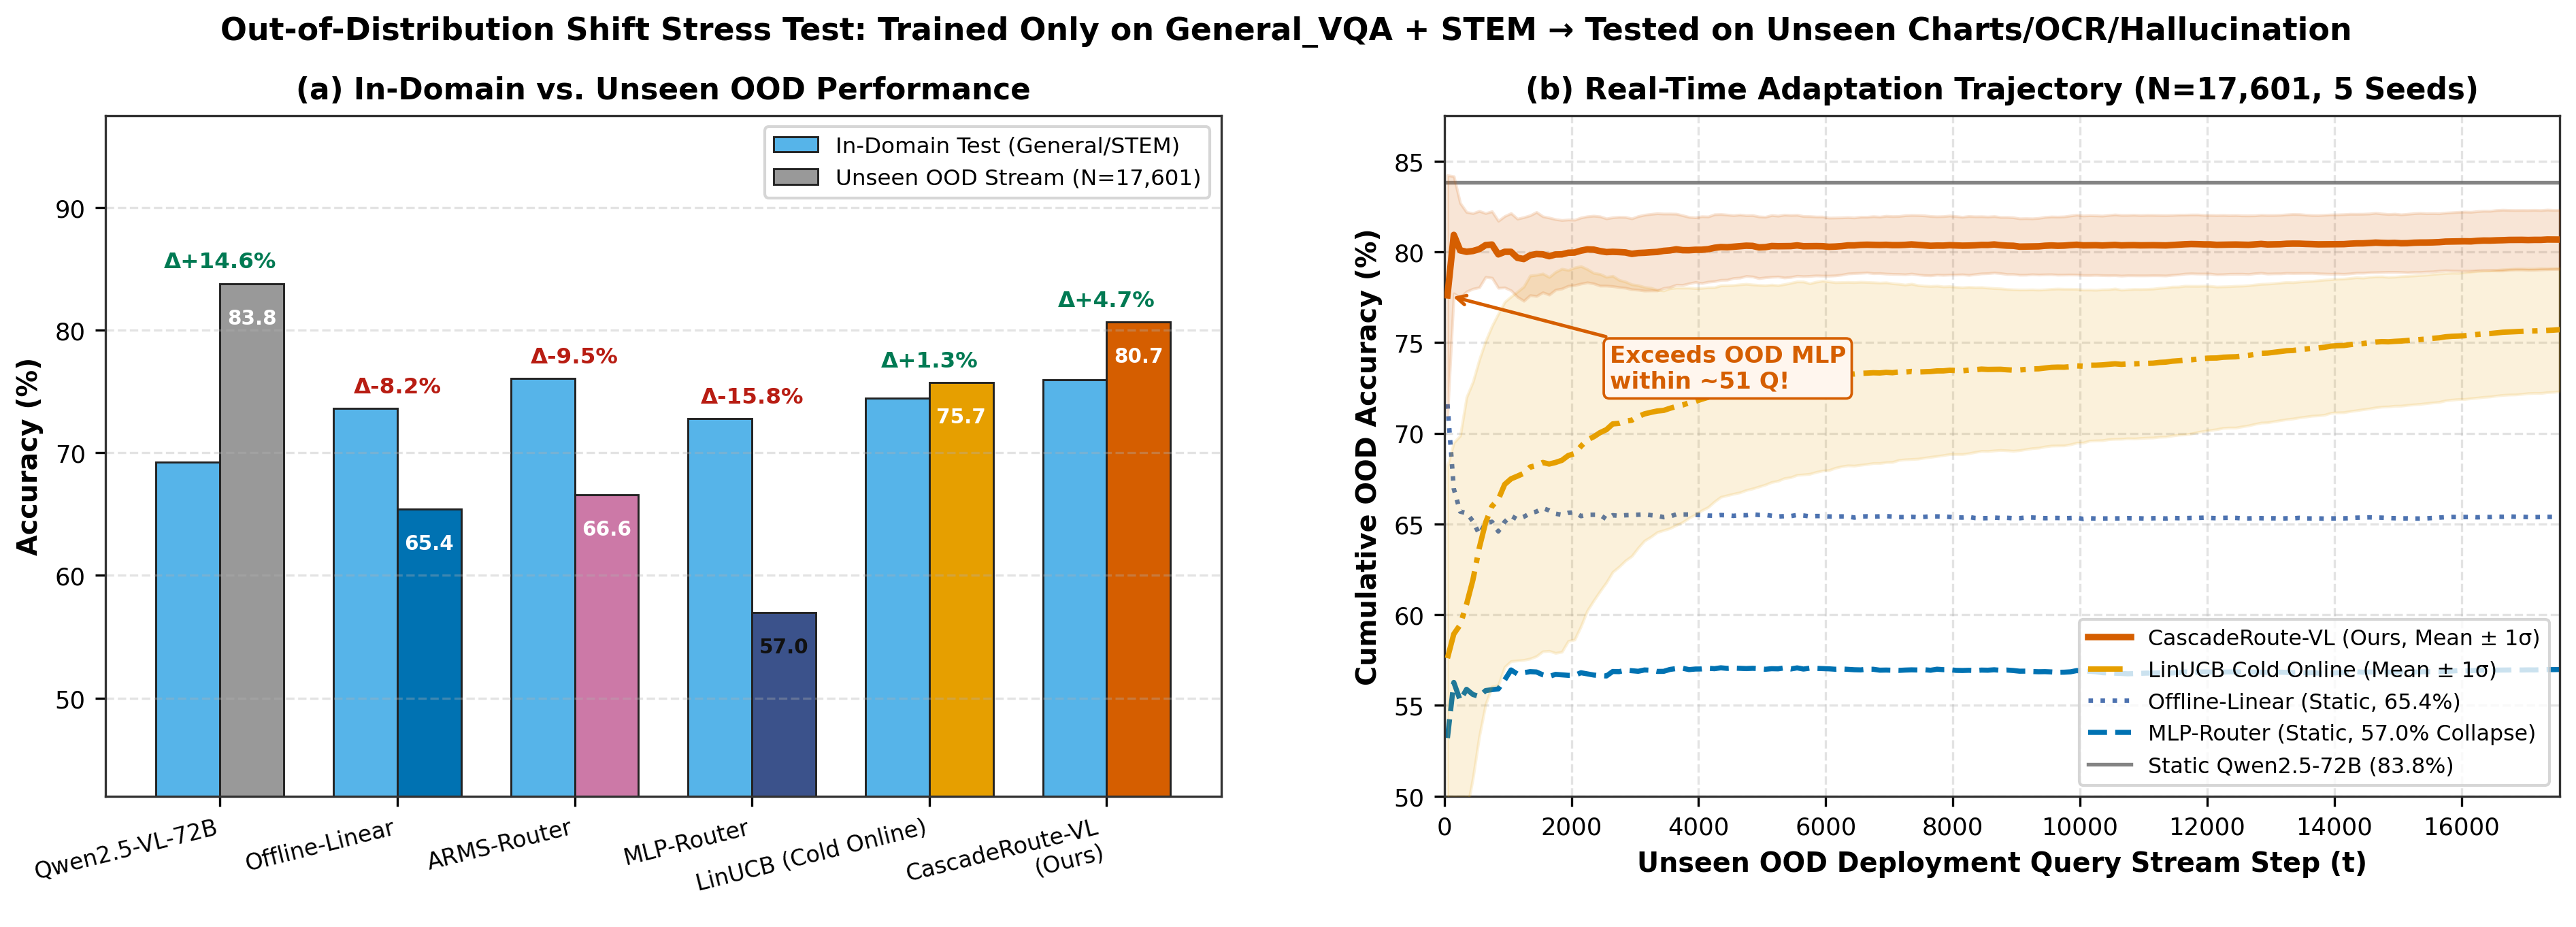
\includegraphics[width=0.87\textwidth]{../reports/figures/fig4_ood_shift_adaptation.png}
\caption{\textbf{Out-of-Distribution Shift Stress Test ($N_{\text{OOD}}{=}17{,}601$, 5 Seeds).} \emph{(a)} Static offline routers collapse moving from \texttt{General+STEM} to unseen OCR/charts (\texttt{MLP-Router}: -15.80\%, \texttt{ARMS}: -9.48\%). \emph{(b)} CascadeRoute-VL surpasses OOD \texttt{MLP-Router} within $\sim$51 queries and reaches 80.68\% (+23.71\% over static MLP).}
\label{fig:ood}
\end{figure*}

Table~\ref{tab:ood} and Figure~\ref{fig:ood} reveal offline fragility vs.\ online plasticity:
\begin{itemize}
    \item \textbf{Offline Collapse:} Frozen \texttt{MLP-Router} relies on reasoning arms that fail or hallucinate on unseen OCR, dropping \textbf{-15.80\%} to \textbf{56.97\%}; \texttt{ARMS} (-9.48\%) and \texttt{Offline-Linear} (-8.24\%) stall below 67\%.
    \item \textbf{Rapid Online Adaptation:} From regularized warm-start ($w_0{=}0.05$), Sherman-Morrison updates surpass OOD \texttt{MLP-Router} within \textbf{$\sim$51 queries} ($4\times$ faster than Cold LinUCB's $\sim$191 Q), reaching \textbf{80.68\%} OOD accuracy (\textbf{+23.71\%} above MLP, \textbf{+4.96\%} above Cold LinUCB).
\end{itemize}

\subsection{Ablations \& Autonomous Domain Specialization}
\label{sec:ablations}

\begin{table}[t]
\centering
\scriptsize
\setlength{\tabcolsep}{2.8pt}
\renewcommand{\arraystretch}{0.94}
\caption{\textbf{Component \& Zero-Label Modality Ablations (Test $N{=}6{,}108$, 5 Seeds).} Warm-start cuts cold exploration cost; perceptual cues lift cold LinUCB by +3.86\%.}
\label{tab:ablations}
\resizebox{\columnwidth}{!}{%
\begin{tabular}{lcccc}
\toprule
\textbf{Ablation Variant} & \textbf{Acc (\%)} & \textbf{Std} & \textbf{Cost / 1k} & \textbf{Cold Acc} \\
\midrule
\multicolumn{5}{l}{\emph{(a) Progressive Component Additions ($\gamma{=}0.08$)}} \\
1. Pure Online LinUCB (Cold) & 72.68 & 1.71 & \$0.3220 & --- \\
2. + Offline Warm-Start Prior & 78.58 & 0.11 & \$0.1590 & --- \\
3. + Budget Annealing ($\alpha_t = \alpha_0 b_t$) & 78.59 & 0.14 & \$0.1591 & --- \\
\textbf{4. + Confidence Gate (Full)} & \textbf{78.59} & \textbf{0.12} & \$0.1598 & --- \\
\midrule
\multicolumn{5}{l}{\emph{(b) Zero-Label Context Modalities ($d$ dims)}} \\
Text Only (MiniLM, 384-d) & 77.82 & 0.23 & \$0.1532 & 70.50 \\
Perceptual Cues Only (8-d) & 77.82 & \textbf{0.07} & \$0.1804 & 66.51 \\
Vision Only (DINO+ResNet, 512-d) & 78.01 & 0.09 & \$0.1563 & 67.87 \\
Vision + Perceptual (520-d) & 77.92 & 0.06 & \$0.1555 & 70.52 \\
Text + Vision Only (896-d) & \textbf{78.77} & 0.16 & \$0.1605 & 68.82 \\
\textbf{Full Joint Multimodal (904-d)} & 78.59 & 0.12 & \$0.1598 & \textbf{72.68} \\
\bottomrule
\end{tabular}%
}
\end{table}

\begin{figure*}[t]
\centering
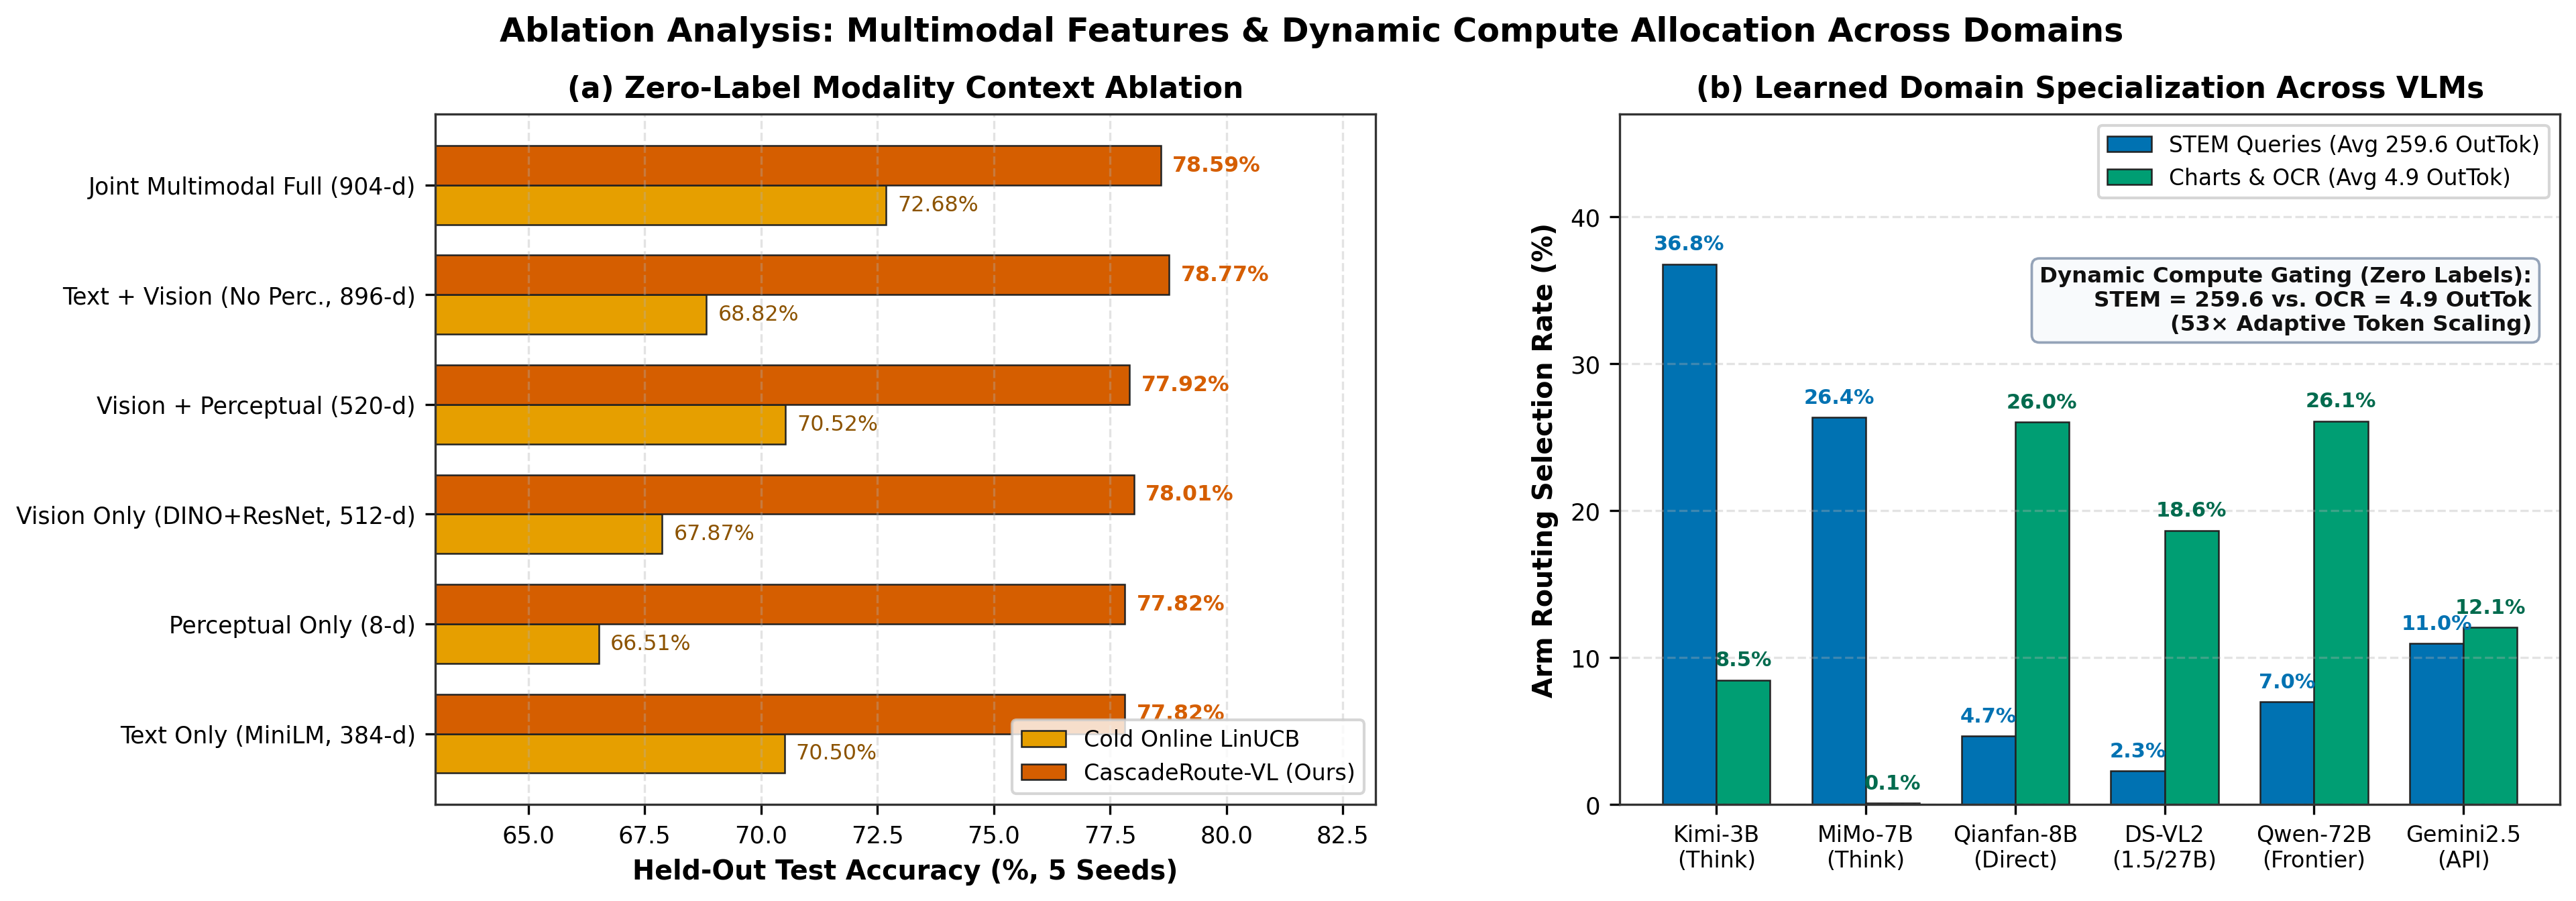
\includegraphics[width=0.87\textwidth]{../reports/figures/fig5_ablations_and_tokens.png}
\caption{\textbf{Modality Feature Ablations and Autonomous Domain Specialization (Test $N{=}6{,}108$).} \emph{(a)} Adding 8 unsupervised perceptual/linguistic cues boosts cold LinUCB from 68.82\% to 72.68\% (+3.86\%) and lowers variance. \emph{(b)} With zero domain labels, CascadeRoute-VL directs STEM traffic to thinking specialists and Charts/OCR to compact perception models (\textbf{53$\times$} token shift: 259.6 vs.\ 4.9).}
\label{fig:ablation}
\end{figure*}

Table~\ref{tab:ablations} and Figure~\ref{fig:ablation} isolate key gains:
\begin{itemize}
    \item \textbf{Component Synergy:} Offline warm-start lifts cold LinUCB by \textbf{+5.90\%} while halving USD cost (\$0.3220 $\to$ \$0.1590/1k). Budget annealing enforces Theorem~2 cleanly; under balanced $\gamma{=}0.08$ the gate escalates 0.25\% of picks, while under frugal $\gamma{=}0.30$ it triggers on \textbf{11.6\%} of ambiguous compact calls (76.13\% @ \$0.0876/1k).
    \item \textbf{Perceptual Cues Value:} Appending 8-d unsupervised cues lifts cold \texttt{Vision-Only} by +2.65\% and cold \texttt{Text+Vision} from 68.82\% to \textbf{72.68\%} (\textbf{+3.86\%}), stabilizing full variance (0.12\%).
    \item \textbf{Zero-Label Emergent Specialization:} Without domain IDs (Fig.~\ref{fig:ablation}b), CascadeRoute-VL routes 63.2\% of \texttt{STEM} queries to thinking arms (\texttt{Kimi-3B-Think} 36.8\%, \texttt{MiMo-VL-RL} 26.4\%, 259.6 out tok; 74.62\% acc vs.\ 67.08\% for 72B), while limiting \texttt{MiMo-VL-RL} to \textbf{0.09\%} on \texttt{Charts\_OCR} and shifting 44.7\% to \texttt{Qianfan-8B}/\texttt{DeepSeek-VL2} (4.9 out tok---\textbf{53$\times$ scaling}).
\end{itemize}

\subsection{Counterfactual Off-Policy Evaluation (OPE)}
\label{sec:ope}

Evaluating stationary policy snapshots over an $\epsilon$-greedy logger ($\epsilon{=}0.50$, $p_0(a|x)\ge 0.50/17$) via IPS, SNIPS~\citep{swaminathan2015self}, and Doubly Robust (DR)~\citep{dudik2011doubly} with 1,000 bootstrap resamples (Table~\ref{tab:ope}), all 95\% CIs closely bracket true on-policy accuracy: for \texttt{CascadeRoute-VL}'s warm-start prior (True \textbf{0.7878}), SNIPS yields \textbf{0.7919} [0.7461, 0.8386] and DR yields \textbf{0.7833} [0.7395, 0.8281] ($\text{ESS}{=}306.4$), confirming finite-sample unbiasedness.

\begin{table}[t]
\centering
\scriptsize
\setlength{\tabcolsep}{2.5pt}
\renewcommand{\arraystretch}{0.94}
\caption{\textbf{Counterfactual Off-Policy Evaluation (Test $N{=}6{,}108$, 1,000 Bootstrap Resamples).} 95\% CIs for IPS, SNIPS, and Doubly Robust (DR) cleanly bracket true on-policy accuracy.}
\label{tab:ope}
\resizebox{\columnwidth}{!}{%
\begin{tabular}{lcccc}
\toprule
\textbf{Policy ($\pi$)} & \textbf{True Acc} & \textbf{IPS (95\% CI)} & \textbf{SNIPS (95\% CI)} & \textbf{DR (95\% CI)} \\
\midrule
\texttt{DS-VL2-Tiny} & 0.6257 & 0.631 [0.520, 0.740] & 0.592 [0.526, 0.663] & 0.576 [0.516, 0.643] \\
\texttt{Qianfan-VL-8B} & 0.6988 & 0.729 [0.615, 0.845] & 0.678 [0.616, 0.742] & 0.696 [0.631, 0.759] \\
\texttt{Qwen2.5-VL-72B} & 0.7729 & 0.844 [0.722, 0.971] & 0.856 [0.810, 0.903] & 0.821 [0.778, 0.866] \\
\texttt{Offline-Linear} & 0.7883 & 0.782 [0.759, 0.805] & 0.784 [0.770, 0.798] & 0.785 [0.771, 0.799] \\
\texttt{MLP-Router} & \textbf{0.7985} & 0.760 [0.665, 0.862] & 0.780 [0.729, 0.827] & 0.774 [0.724, 0.820] \\
\textbf{CascadeRoute-VL} & 0.7878 & \textbf{0.836} [0.733, 0.937] & \textbf{0.792} [0.746, 0.839] & \textbf{0.783} [0.740, 0.828] \\
\bottomrule
\end{tabular}%
}
\end{table}

% ============================================================================
\section{Discussion, Limitations, and Conclusion}
\label{sec:conclusion}
% ============================================================================

\textbf{Limitations \& Transparency.} (1)~On \texttt{ChartQA}, \texttt{DocVQA}, \texttt{InfoVQA}, and \texttt{TextVQA}, upstream \texttt{MiMo-VL-7B-RL} transcripts record 0.0\% extracted accuracy as unclosed \texttt{<think>} tags break parsing; CascadeRoute-VL avoids this cleanly (0.09\% OCR rate). (2)~Latencies follow deterministic TTFT+throughput profiling on exact \texttt{cl100k\_base} tokens rather than queueing jitter; USD savings reflect published token pricing. (3)~Feature extraction takes $\sim$2--4\,ms/query on GPU, negligible vs.\ multi-second 72B decoding.

\textbf{Conclusion.} We introduced \textbf{CascadeRoute-VL}, a zero-leakage online contextual bandit resolving the Multimodal Reasoning Tax across 30,540 queries, 14 benchmarks, and 17 VLMs. Fusing a bounded 904-d perceptual state, warm-started Sherman-Morrison LinUCB, budget annealing, and confidence-guided escalation, it beats static 72B models while saving 38.7\%--66.4\% USD, scaling compute 53$\times$ without labels, and adapting in $\sim$51 unseen OOD queries where offline routers collapse.

\FloatBarrier
{\small
\bibliographystyle{ieeenat_fullname}
\bibliography{references}
}

\end{document}
